\section{Experiment}\label{sec:experiment}
In section~\ref{sec:training}, we have shown the model accuracy and epoch consumption of the proposed hardware friendly training process. In this section, we show the hardware experimental results. A prototype design is implemented on a Xilinx XCKU115 chip with 2 on-board DDR4 SDRAM. In this system, feature map, neuron and their gradients are all of 8-bit and stored in DDR0. Network weights, each of which includes 8-bit MSB for computation and 24-bit LSB buffer, are stored in DDR1. Corresponding index for sparse representation are stored in DDR0 using \{y[3:0], x[3:0]\} format. This means the the maximum weights block size can be $16\times 16$. The system operates at 200MHz. Each $2\times 2$ PEs are grouped together for CONV layers.

\begin{table}[tb]
  \centering
  \caption{Prototype design resource utilization}
    \begin{tabular}{|c|c|c|c|c|}
    \hline
    Resource & LUT   & Reg   & Block RAM & DSP \\
    \hline
    Available & 663360 & 1326720 & 2160  & 5520 \\
    \hline
    Utilization & 193821 & 144594 & 1216   & 1024 \\
    \hline
    Ratio & 29\%  & 11\%  & 56\%  & 19\% \\
    \hline
    \end{tabular}
  \label{tab:util}
\end{table}

\subsection{Effect of Workload Imbalance}\label{sec:exp:imb}

Before introducing the hardware performance, we first analyze the theoretical performance loss brought by workload imbalance in Table~\ref{table:sparsity}. As introduced in section~\ref{sec:hw_unroll}, unroll parameters are limited by loop dimension variety and sparsity. As we cannot group the PEs for fully connected layers, we only compare on the convolutional layers. The normalized speed on the convolutional layers of each configuration is shown in Table~\ref{tab:hw_util}.

\begin{table}[tb]
  \centering
  \caption{Comparison of PE utilization with different group sizes on a network}
    \begin{tabular}{|c|c|r|r|r|r|r|}
    \hline
    \multirow{2}[4]{*}{Layer} & Feature & Workload & \multicolumn{3}{c|}{Utilization} \\
\cline{4-6}          & size & (MOP) & Single & 2x2 & Ideal\\
    \hline
    conv1 & $32\times 32$ & 3.54 & 80    & 88.5  & 100\\
    \hline
    conv2 & $16\times 16$ & 151 & 88.6  & 95.8  & 100\\
    \hline
    conv3\_1 & $8\times 8$   & 37.7 & 95.1  & 98.2  & 100\\
    \hline
    conv3\_2 & $8\times 8$   & 75.5 & 96.4  & 98.8  & 100\\
    \hline
    conv4\_1 & $4\times 4$   & 37.7 & 96.3  & 98.7  & 100\\
    \hline
    conv4\_2 & $4\times 4$   & 75.5 & 95.6  & 98.4  & 100\\
    \hline
    conv5\_1 & $2\times 2$   & 18.87 & 93.5  & 97.8  & 100\\
    \hline
    conv5\_2 & $2\times 2$   & 18.87 & 93.5  & 97.8  & 100\\
    \hline
    \multicolumn{3}{|c|}{Normalized Speed} & 1     & 1.050 & 1.078 \\
    \hline
    \end{tabular}
  \label{tab:hw_util}
\end{table}

\begin{figure}[tb]
  \centering
  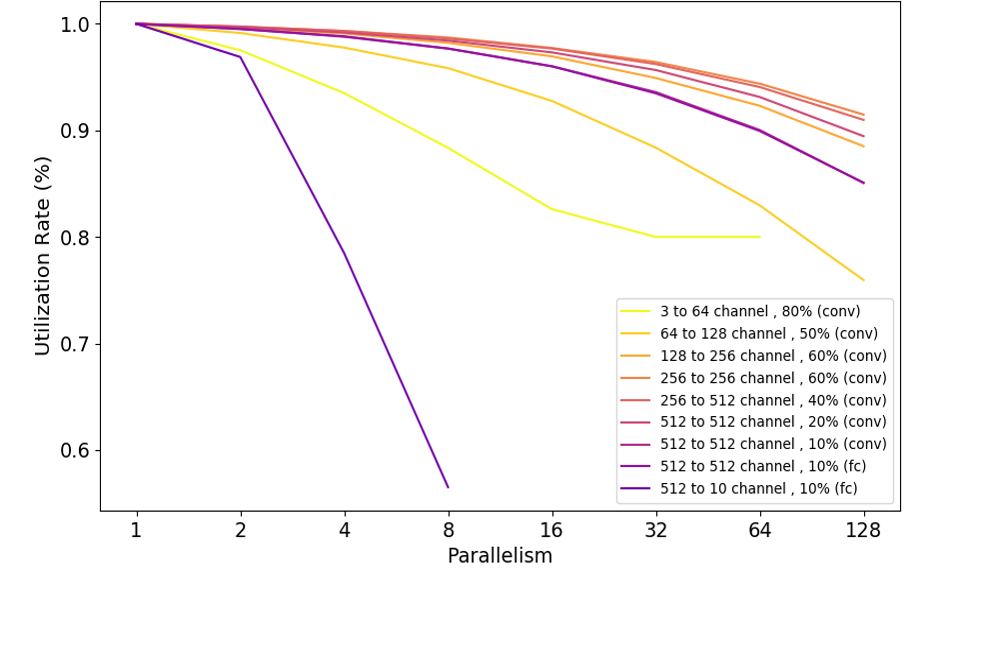
\includegraphics[width=1.0\columnwidth]{figures/util_real.png}
  \caption{Theoretical utilization ratio for each layer over the number of PEs.}
  \label{fig:util_real}
\end{figure}

Here, we see that using 32 PEs for this network will suffer from $7\%$ performance loss compared with the ideal case where no workload imbalance occurs. Group each 4 PEs together brings about $5\%$ performance increase. %Figure~\ref{fig:util_real} shows the utilization ratio of each layer over the number of PE(PE groups). The performance loss in the second layer contributes the most. Further increase the number of PEs will 


\subsection{Hardware Performance}
We simulate the performance of each layer in each training step with the DDR model and controller from Xilinx IP. Detailed running time and performance are shown in Table~\ref{tab:layerperformance}.

% Table generated by Excel2LaTeX from sheet 'Sheet4'
\begin{table*}[tb]
  \centering
  \footnotesize
  \caption{The performance of each layer. \textit{Comp.} indicates the complexity of each layer. \textit{Perf.} indicates the performance of running each layer on our hardware. \textit{Bound type} indicates the performance of each layer is bounded with bandwidth (B) or computation (C).}
% Table generated by Excel2LaTeX from sheet 'Sheet4'
\begin{tabular}{|c|c|c|c|c|c|c|c|c|c|c|c|c|c|}
\hline
      &       & \multicolumn{4}{c|}{Feed Forward (FF)}  & \multicolumn{4}{c|}{Neuron Gradient(NG)} & \multicolumn{4}{c|}{Neuron Gradient(NG)} \bigstrut\\
\cline{2-14}layer & Comp. & Time  & Perf. & bound & Utilize & Time  & Perf. & bound & Utilize & Time  & Perf. & bound & Utilize \bigstrut[t]\\
      & (GOP) & (us)  & (GOP/s) & type  & rate  & (us)  & (GOP/s) & type  & rate  & (us)  & (GOP/s) & type  & rate \bigstrut[b]\\
\hline
conv1 & 0.11  & 733   & 154.4  & B     & 27\%  & -     & -     & -     & -     & 4158  & 27.2  & B     & 5\% \bigstrut\\
\hline
conv2 & 1.21  & 1487  & 812.2  & C     & 95\%  & 1487  & 812.5  & C     & 95\%  & 2804  & 430.8  & B     & 50\% \bigstrut\\
\hline
conv3\_1 & 1.21  & 1696  & 712.4  & C     & 97\%  & 1694  & 713.0  & C     & 97\%  & 2477  & 487.7  & B     & 67\% \bigstrut\\
\hline
conv3\_2 & 2.42  & 2877  & 839.7  & C     & 98\%  & 2876  & 840.1  & C     & 98\%  & 4398  & 549.3  & B     & 64\% \bigstrut\\
\hline
conv4\_1 & 1.21  & 1217  & 992.3  & C     & 97\%  & 1217  & 992.9  & C     & 97\%  & 2686  & 449.8  & B     & 44\% \bigstrut\\
\hline
conv4\_2 & 2.42  & 1457  & 1658.4  & C     & 97\%  & 1456  & 1659.2  & C     & 97\%  & 3933  & 614.2  & B     & 36\% \bigstrut\\
\hline
conv5\_1 & 0.60  & 366   & 1651.7  & B     & 32\%  & 358   & 1687.7  & B     & 33\%  & 915   & 659.8  & B     & 13\% \bigstrut\\
\hline
conv5\_2 & 0.60  & 365   & 1652.7  & B     & 32\%  & 358   & 1688.7  & B     & 33\%  & 915   & 660.0  & B     & 13\% \bigstrut\\
\hline
dense6 & 0.02  & 329   & 51.0  & B     & 1\%   & 328   & 51.1  & B     & 1\%   & 717   & 23.4  & B     & 0.5\% \bigstrut\\
\hline
dense7 & 0.02  & 329   & 51.0  & B     & 1\%   & 328   & 51.1  & B     & 1\%   & 717   & 23.4  & B     & 0.5\% \bigstrut\\
\hline
dense8 & 0.003  & 75    & 4.4   & B     & 0.1\% & 74    & 4.4   & B     & 0.1\% & 272   & 1.2   & B     & 0.02\% \bigstrut\\
\hline
total & 9.81  & 10931  & 897.5  & -     & -     & 10988  & 892.8  & -     & -     & 23993  & 408.9  & -     & - \bigstrut\\
\hline
\end{tabular}%
  \label{tab:layerperformance}%
\end{table*}%

% Table generated by Excel2LaTeX from sheet 'Sheet4'
\begin{table*}[tb]
  \centering
  \caption{Performance and energy efficiency comparison with GPU. }
    \begin{tabular}{|c|c|c|c|c|c|c|c|}
    \hline
          & Data Format & Forward time & Backward time & Total time & Performance & Power & Power efficiency \bigstrut[t]\\
          & data+gradiant & (us)  & (us)  & (us)  & (GOP/s) & (W)   & (GOP/s/W) \bigstrut[b]\\
    \hline
    GPU   & float + float & 7795  & 15700  & 23495  & 1252.7  & 150   & 8.4  \bigstrut\\
    \hline
    FPGA  & 8bit + 24bit & 10931  & 34981  & 45912  & 641.1  & 29    & 22.1  \bigstrut\\
    \hline
    \end{tabular}%
  \label{tab:exp_comp}%
\end{table*}%

The peak performance of the hardware is $250MHz \times 1024DSP \times 2 = 500GOP/s$. For FF and NG steps, the proposed hardware achieves 900GOP/s overall performance which achieves at least $1.8\times$ speedup over a dense accelerator with the same peak performance. From the bound type column, we see that most of the CONV layers with heavy workload are computation bounded. This shows that the proposed accelerator can handle large network well.

A performance and energy efficiency comparison is shown in Table~\ref{tab:exp_comp}. The GPU used for comparison is GTX Titan X GM200. Alough GPU achieves about 2x speed compared with FPGA, the FPGA part only consumes 1/5 power compared with GPU and achieves 3x energy efficiency.

Besides that, those layers which are bandwidth bounded gives insights to hardware design methods. The first layer suffers from the bandwidth problem because the channel number for this layer is small. We only cut $3\times 8$ block for this layer. A small block size increases the ratio between the necessary feature maps and the necessary convolution kernels. Compared with the workload imbalance result in \ref{sec:exp:imb}, we see that small layers suffer more on bandwidth rather than workload imbalance. Besides reducing the number PEs, increase the buffer size in PEs can help further explore the data locality of 2-d convolution and improves performance. 

The last few layers also suffers greatly from a limited bandwidth. On the one hand, FC layers and convolution layers with small feature maps are of high bandwidth cost for network parameters. On the other hand, split the parameters into small blocks decreases the memory access efficiency. Increase the the 

When upgrading the weights of each layer, the weight buffer consumes more bandwidth and causes the performance loss. Reduce the weight buffer size should also be a future research topic. 





